\chapter{Sistema propuesto: teoría y simulaciones}

Se propone un sistema de comunicaciones punto a punto y punto a multipunto de medio compartido también denominado de broadcast. En la figura \ref{fig_hub} se aprecia su estructura lógica del sistema, que en la versión óptica equivale a una red de tipo estrella con un hub amplificador central, pero utilizando diferentes medios esta configuración puede cambiar (Por ejemplo, puede no ser necesaria la etapa de amplificación).
Al ser un sistema de tipo TDMA o time-hopping, cada cliente puede utilizar el medio por un intervalo determinado de tiempo denominado slot. Esto permite utilizar el medio para múltiples clientes asignando a cada uno un slot diferente. La diferencia del sistema propuesto con un sistema TDMA regular en donde el slot es asignado a cada cliente de manera periódica, en el sistema propuesto el slot se asigna mediante un algoritmo CS-PRNG. Esto tiene dos efectos fundamentales: 

\begin{itemize}
 \item Un atacante no puede predecir la posición en donde un cliente en particular transmite los datos. En particular, si el slot se reduce al mínimo de un solo bit por slot, el atacante no puede inferir ninguna información acerca de los datos transmitidos sin conocer los parámetros del algoritmo CS-PRNG.
 \item Existirá una inevitable interferencia entre los clientes, lo que requiere la utilización de algoritmos de corrección de errores.
\end{itemize}

Como se describe en el capítulo \ref{PRNGs}, existen varios algoritmos de generación de números pseudo aleatorios criptográficamente seguros estandarizados, cuya mayor dificultad es la implementación sobre silicio de manera eficiente. Esta tesis no ahonda sobre el tema y nos limitaremos a indicar que puede seleccionarse cualquiera mientras sea un algoritmo estandarizado por la industria y no posea ninguna vulnerabilidad conocida. Otra virtud que debe poseer el algoritmo seleccionado es una alta relación de bits generados por unidad de tiempo o clock, ya que al ser utilizados para seleccionar la posición de cada bit en el frame, se necesitan $\log_2(M)$ bits aleatorios por cada bit de datos, por lo que en general la velocidad del PRNG afectara directamente la velocidad total de codificación y decodificación del sistema.

El aporte mas importante de esta tesis es en la etapa de corrección de errores, ya que se necesitó desarrollar algoritmos adaptados al medio de transmisión y a la gran cantidad de interferencia producida por el método aleatorio de selección de slot de transmisión.

%Utilizando este Diseño físico con una etapa adicional de codificación y correccion de errores. El hub central es una etapa totalmente óptica que puede o no estar amplificada. Con la amplificacion optica se incrementa notablemente el rango, de 5 km a mas de 20 km.
La pila de codificación se detalla en la figura \ref{fig_comstack} donde se aprecia un diseño convencional, excepto que en la ultima etapa de corrección de errores se aplica el algoritmo de filtros de Bloom, que aprovecha la característica de error asimétrico del canal Z para una corrección de errores adicional.

\begin{figure}[t]
\centering
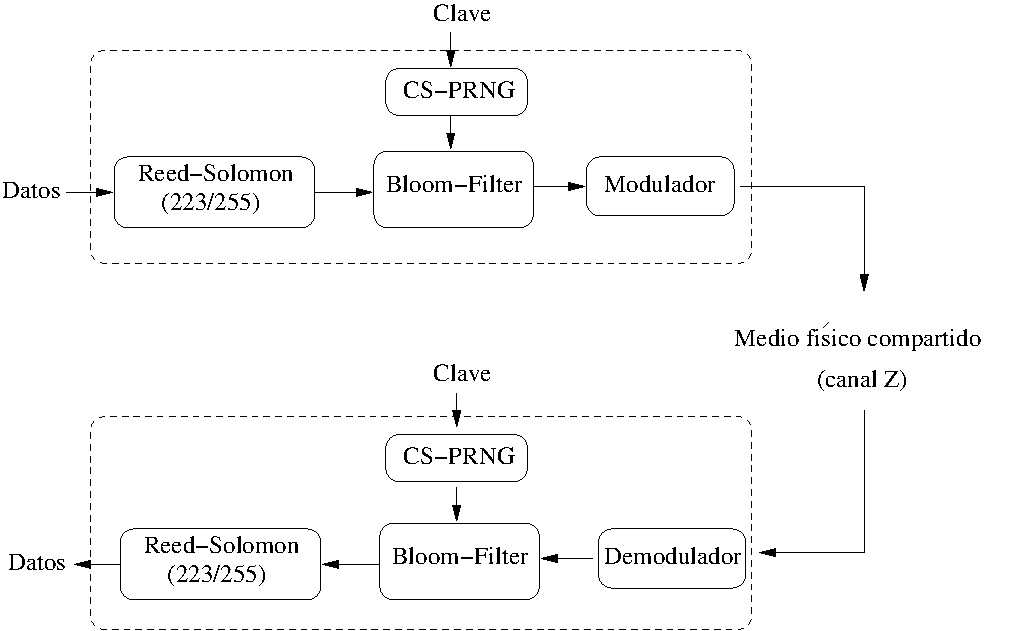
\includegraphics[width=4.5in]{graphs/Soft-stack3}
\caption{Etapas del sistema de comunicaciones}
\label{fig_comstack}
\end{figure}

\section{Códigos correctores de errores}

La selección del código corrector de errores debe ser guiada por los parámetros del sistema, sin olvidarse de las posibles limitaciones de calculo del sistema, que es una limitación importante al operar con enlaces con tasas de transmisión elevadas.

En nuestro caso se utilizó un típico arreglo de dos códigos de corrección, uno denominado exterior, encadenado con el segundo denominado interior.
La idea de utilizar dos códigos distintos es la de aprovechar las virtudes de dos tipos de corrección. El código exterior suele ser un código iterativo o convolucional, con una elevada cantidad de paridad y alto poder de detección y corrección. Ciertos tipos de códigos tales como LDPC o códigos Turbo se caracterizan por poseer un piso de error elevado, que es un fenómeno en donde el código pierde efectividad con SNR altos. Esto se soluciona utilizando un segundo código corrector denominado interior, que si bien no es tan efectivo a SNR altos como el código exterior, es efectivo con SNR bajos, haciendo que el sistema sea efectivo en cualquier condición.

Un parámetro importante en estos algoritmos es el delay, o sea la cantidad de tiempos (medida usualmente en clocks del procesador) que tarda un bit que entra a la etapa de corrección en salir de la misma, luego de la aplicación de la corrección. Este delay es variable según el algoritmo, algunos algoritmos con un delay importante no pueden ser utilizados en aplicaciones de bajo ancho de banda, ya que retrasan enormemente las comunicaciones. A continuación se detalla el algoritmo de corrección seleccionado.

\subsection{Reed-Solomon}
Como código interior se seleccionó el algoritmo Reed-Solomon, un código de bloque con alta efectividad en SNR bajos. Los parámetros seleccionados para dicho código son (255,223) o sea, 223 bytes de datos y 32 bytes de paridad. Estos parámetros lograran que el código pueda detectar hasta 32 errores de byte y corregir hasta 16 errores de byte en los 223 bytes del bloque. La selección de estos parámetros responde a que el algoritmo de Reed-Solomon posee implementaciones muy eficientes si se utiliza un tamaño de bloque de 255 bytes. 
Al ser un estándard muy utilizado, existen implementaciones muy eficientes de Reed-Solomon con estos parámetros específicos, tanto en software como en hardware.
Existen dos problemas con este algoritmo:
\begin{enumerate}
 \item Elevado delay: Si bien el delay de codificación es mínimo (menos de 10 clocks), el delay de decodificación es muy elevado, pudiendo sobrepasar fácilmente los 1200 clocks.
 \item Si bien el delay de decodificación es elevado y requiere mucho procesamiento, el solo echo de tener que acumular un bloque de 256 bytes de datos solo para comenzar con la decodificación, introduce un retraso muy importante especialmente si el sistema se utiliza con bajo ancho de banda, tal como es el caso en la implementación acústica del sistema.
\end{enumerate}
 
Ambos problemas se solucionan seleccionando parametros de Reed-Solomon con un menor tamaño de bloque, o un algoritmo similar con menor tamaño de bloque tal como BCH. El problema en este caso es encontrar implementaciones eficientes de los decodificadores ya que no son algoritmos muy utilizados, por lo que la selección final fue el estandard Reed-Solomon (255, 223).

Para la simulación numérica por software se utilizó la biblioteca libfec de Phil Karn~\cite{libfec}. Para la implementación en FPGA se utilizo la versión del algoritmo provista de manera gratuita en la biblioteca de núcleos de IP de Xilinx.

%Con posibilidad de error de simbolo P, la posibilidad de error de un codigo reed-solomon R(n/k) es:
%$$P_{rs}= \sum_{k=(\frac{n-k}{2}+1)}^{n} \binom{L}{i} * P^{i} * (1-P)^{L-i} $$
El código (255,223) es particularmente eficiente de implementar digitalmente ya que cada símbolo puede representarse con un byte (existen 255 símbolos). El código posee 32 bytes de paridad y 223 bytes de datos, lo que representa una adición de 14\% a la cantidad total de datos a transmitir. Este código permite corregir hasta 16 bytes errados, que pueden estar consecutivos, por lo que RS suele utilizarse en canales con errores de tipo ``Erasure'' o errores tipo ráfaga, donde los errores no están uniformemente distribuidos sino que están agrupados temporal o espacialmente.

%En ciertas ona ventaja muy importante es que el codigo de correccion exterior puede facilmente detectar la presencia de un error aunque no pueda corregirlo. Esta informacion es una lista con las posiciones en las cuales se tiene la certeza que los símbolos fueron interferidos denominada lista de síndromes, y puede suministrarse al algoritmo de correccion de errores para que la capacidad de corrección del mismo puede aumentar hasta un 100\%~\cite{Moon:05}.

\subsection{Características de implementación}
Un parámetro importante en la selección del algoritmo es la facilidad de implementación sobre hardware digital. Ciertas características se vuelven importantes al pasar de implementaciones de software a hardware, tales como tamaño, memoria utilizada y velocidad máxima alcanzada con el hardware disponible, apuntando a que el sistema debe funcionar a tasas de gigabit.

A continuación se nombraran las características de la implementación en hardware (FPGA) de Reed-Solomon utilizada.
El bloque de IP se denomina Reed-Solomon Encoder/Decoder 7.1 de LogiCORE IP. La complejidad espacio-temporal y ciclomática de los algoritmos de codificación de Reed-Solomon son muy distintas a las de su correspondiente algoritmo de decodificación. En general, la decodificación es mucho mas costosa en términos de recursos de hardware y de latencia agregada al sistema.

Según la especificación de esta implementación~\cite{Xilinx:DS252} el decodificador Reed-Solomon con configuración CCSDS (que implementa el estandard (255,223)) posee un tamaño de 1364 LUTS (Look-up tables) y 3 bloques de RAM. Como comparación, el diseño completa posee un tamaño de aprox. 20000 LUTS, y la FPGA utilizada posee una capacidad de 50000 LUTS y unos 200 bloques de RAM. La velocidad máxima de este algoritmo en la FPGA utilizada es de unos 350 Mhz.
Mucho menor es la cantidad de recursos utilizados por el codificador: Son necesarios solo unos 300 LUTS y solo 1 bloque de memoria aunque la velocidad máxima es similar~\cite{Xilinx:DS251}.

\subsection{Cálculo de latencia}
La latencia en un sistema esta dada por el tiempo en que un bit tarda en atravesarlo en su totalidad. Específicamente la latencia de esta etapa es importante ya que la latencia agregada por este algoritmo representa un porcentaje importante de la latencia total de la pila de comunicación del sistema. Es importante notar que los cálculos son específicos de una implementación en particular. 

La latencia total estará dada por la introducida por la codificación adicionada a la de la decodificación ya que los datos deben atravesar ambas etapas. Pero los tiempos de latencia para la codificación son despreciables, en el orden de 5 clocks. 

La latencia de la etapa de decodificación es muy superior y puede ser calculada de manera exacta mediante ecuaciones provistas por la hoja de datos. Una manera simplificada es utilizar la figura \ref{fig_rslat} para obtener el delay de procesamiento. El parámetro $t$ se calcula como $t=(n-k)/2$ donde $n$ es la cantidad de símbolos totales en el bloque (en nuestro caso 255) y $k$ es la cantidad de símbolos de datos en el bloque (223 en nuestro caso) por lo que la variable $t=16$.  El retraso total introducida por la decodificación estará dada por la latencia (en nuestro caso aprox. 650 clocks) mas el retraso producto de cargar un bloque entero de datos en el decodificador, que no es despreciable ya que deben ingresarse los datos al bloque IP por medio de un bus serial de un byte de capacidad, por lo que se necesitan de 255 clocks adicionales por cada bloque. 

Sumando ambos valores e ignorando la mínima latencia de codificación, podemos afirmar que la latencia introducida por el algoritmo Reed-Solomon en el sistema es de 900 clocks.

\begin{figure}[t]
  \centering
  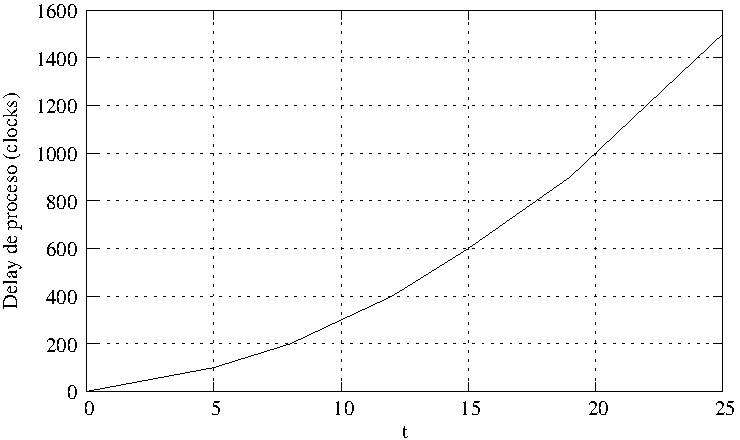
\includegraphics[width=0.6 \textwidth]{graphs/rsDelay.pdf} 
  \caption{Delay de proceso de la implementación de Reed-Solomon utilizada.}
  \label{fig_rslat}
\end{figure}


\subsection{Optimizaciones propuestas}
 
Existen ciertas optimizaciones que podrían haberse realizado si se hubiera optado por implementar el algoritmo desde cero, pero que al utilizar una implementación pre-existente no se realizaron. Estas optimizaciones están relacionadas con la características del canal asimétrico, que presenta las ventajas de tener la certeza de que ciertos símbolos fueron transmitidos correctamente. Una posible optimización de Reed-Solomon para su utilización sobre canales Z se plantea para una trabajo futuro.

\section{Canal Z con filtros de bloom}

En esta sección vamos a modelar el canal por el cual estamos transmitiendo datos, específicamente el modelo de ruido del mismo. 
Un canal de comunicaciones puede clasificarse primeramente según el tipo de información transmitida, sea binaria o analógica, por lo cual tendremos canales binarios o analógicos \cite{MacKay:2002}.
Una sub-clasificación del canal de comunicación puede realizarse según el comportamiento del ruido del mismo.
Por ejemplo las comunicaciones por radiofrecuencia suelen modelarse como un canal analógico AWGN (Additive White Gaussian Noise). 

Específicamente, un canal digital suele clasificarse como canal discreto sin memoria (Discrete memoryless channel), ya que posee un alfabeto de símbolos de entrada $A_{x}$, que son los datos que se desea transmitir, y un alfabeto de símbolos de salida $A_{y}$ , que son los símbolos actualmente detectados por el receptor. El canal es discreto ya que la cantidad de símbolos posible es finita. Los datos a transmitir deberán codificarse en el alfabeto de símbolos de entrada.
Otro parámetro importante que define a un canal discreto es la distribución de probabilidades condicionales $P(y|x)$ entre ambos alfabetos, o sea la posibilidad de que al recibir el símbolo $x$ se haya transmitido el símbolo $y$. Esta distribución puede representarse como un diagrama (ver figura \ref{fig:canbin} para la representación de distribución de probabilidades de un canal binario simétrico) o una matriz.

De acuerdo con la distribución de probabilidades de error que mejor represente al canal físico de transmisión, 
El tipo de canal que mejor modela las transmisiones digitales por fibra óptica es el denominado canal Z (Z-Channel), un canal digital en el que el ruido afecta solo uno de los símbolos a transmitir.

Es este modelo de ruido lo que nos permite innovar en el diseño de algoritmos adaptándolos y optimizándolos para aprovechar la naturaleza del error, ya que la mayoría de los algoritmos de corrección de errores están pensados para un canal de ruido simétrico y generalmente analógico.
Empezaremos primeramente estudiando un modelo simplificado del canal por el cual vamos a trasmitir, el mencionado canal simétrico binario, para después ahondar en un caso especial de este mismo, denominado Canal Z.

\section{Probabilidad de error de canal binario simétrico}

\begin{figure}[t]
  \begin{center}
    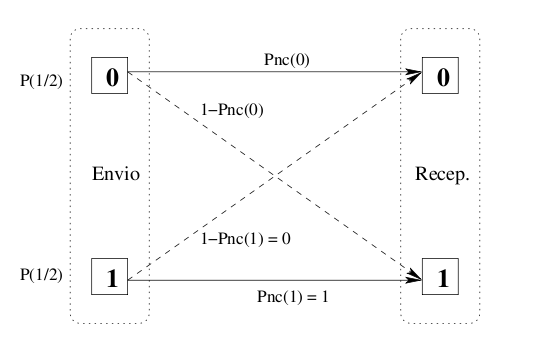
\includegraphics[scale=0.43]{capacidad/canalBinario.png}
  \end{center}
\caption {Canal binario: esquema de probabilidad}
\label{fig:canbin}
\end{figure}

Para calcular el ruido en un canal simétrico binario, calculamos la probabilidad de no-colisión que tendrá un usuario determinado, ya que las colisiones serán el ruido del canal (En esta etapa no consideramos otros tipos de ruido que pueda tener el canal físico).

Sea $M$ la cantidad de slots por frame y $n$ la cantidad de clientes o usuarios.

Entonces la probabilidad de no colisión para un usuario en un canal simétrico esta dada por:
\begin{equation}
P_{nc}=\left(\frac{M-1}{M}\right)^{n-1}
\end{equation}


\noindent Probabilidad de no colisión para un usuario en un canal Z:
\begin{eqnarray}
P_{nc} & = & P(1) \cdot P_{nc}(1) + P(0) \cdot P_{nc}(0) \\
P_{nc} & = & \frac{1}{2} \cdot 1 +  \frac{1}{2} \cdot \sum_{i=0}^{n-1} 
C^{n-1}_{i} \left(\frac{M-1}{M}\right)^i  \left(\frac{1}{M}\right)^{n-1-i}  \left(\frac{1}{2}\right)^{n-1-i} 
\end{eqnarray}

\noindent Donde $\left(\frac{M-1}{M}\right)^i$ es la probabilidad de no colisión de $i$ canales (se suma para todo posible número de canales no
colisionando: $1\leq i\leq n$, que están en otro slot), $
\left(\frac{1}{M}\right)^{n-1-i}$ es la probabilidad de colisión de los restantes
$n-1-i$ (estos están en el mismo slot que el canal actual, el `$-1$' es para no
contar el canal actual), y la colisión se produce cuando los otros canales
transmiten $1$ cuya probabilidad es $\left(\frac{1}{2}\right)^{n-1-i}$. El
factor $C^{n-1}_{i}$ suma sobre todas las combinaciones posibles de canales no
colisionando, que son hechos independientes.

\noindent Teniendo en cuenta que $ \sum_{i=0}^{n-1}
C^{n-1}_{i} \left(\frac{M-1}{M}\right)^i  \left(\frac{1}{2M}\right)^{n-1-i}$ es la potencia $n-1$ de un binomio, reemplazando tenemos
\begin{eqnarray}
P_{nc} & = & \frac{1}{2} +  \frac{1}{2} \cdot \left(\frac{M-1}{M} + \frac{1}{2M} \right)^{n-1} \\
P_{nc} & = & \frac{1}{2} +  \frac{1}{2} \cdot \left(1- \frac{1}{2M} \right)^{n-1} \\
P_{nc} & \simeq & \frac{1}{2} +  \frac{1}{2} \cdot e^{-1/2} REVISAR ESTO
\end{eqnarray}

\noindent Donde la última aproximación vale para $n=M$ y $n$ grande.

\iffalse

\vspace{5mm}

\noindent Para el caso de {\em bloom} filters con $k$ filtros\footnote{Se envían $k$ repeticiones del bit en canales distintos, entonces basta que sólo uno de ellos sea 0 para que recibamos un 0 en un canal óptico.} la probabilidad de no colisión es:
\begin{eqnarray} 
P_{nc}^{k} & = &  P(1) \cdot P_{nc}^{k}(1) + P(0) \cdot P_{nc}^{k}(0)\\ \label{Pnc_k}
\end{eqnarray}
Sabiendo que la probabilidad de no colisión para el 0 es:
\begin{eqnarray}
P_{nc}^{k}(0) & = & 1 - \big(P_{c^k}(0)\big)^k 
\end{eqnarray}
Pero la probabilidad de colisión para el 0 cuando se transmiten $k$ copias es:
\begin{eqnarray}
P_{c^k}(0) & = & 1 - \big(P_{nc^k}(0)\big)  \enspace,
\end{eqnarray}
y que además la probabilidad de no colisión para los $k$ slots del bloom
filter es
\begin{eqnarray}
P(\mbox{no col.} k) &=& P(\mbox{no col.}1)\cdot P(\mbox{no col.}2)\cdot P(\mbox{no col.}3)\cdots P(\mbox{no col.}k)\\
&=&\left(\frac{m-1}{m}\right)\cdot\left(\frac{m-2}{m-1}\right)\cdot\left(\frac{m-3}{m-2}\right)\cdots\left(\frac{m-k}{m-(k-1)}\right)\\
&=& \frac{m-k}{m} \enspace.
\end{eqnarray}
Luego la probabilidad de colisión con alguno de las $k$ copias del bit es
\begin{eqnarray}
P(\mbox{col.}k)&=& 1-P(\mbox{no col.} k)\\
&=& 1-\frac{m-k}{m}\\
&=& \frac{k}{m} \enspace.
\end{eqnarray}
Entonces reemplazamos y calculamos:
\begin{eqnarray}
P_{c^k}(0) & = & 1 - \left(\sum_{i=0}^{n-1} C^{n-1}_{i} \left(\frac{m-k}{m}\right)^i \left(\frac{k}{2m}\right)^{n-1-i} \right)  \\
& = &  1-\left( 1-\frac{k}{2m}\right)^{n-1}
\end{eqnarray}
Reemplazando esta ecuación en~\ref{Pnc_k} obtenemos:
\begin{eqnarray}
P_{nc}^k & = & \frac{1}{2} + \frac{1}{2} \left( 1- \left( 1- \left( 1- \frac{k}{2m} \right)^{n-1}  \right)^{k}  \right) 
\end{eqnarray}

Sin embargo, este calculo es incorrecto, comparandolo con los datos que da el simulador. La formula entrega valores de error menores con respecto a los reales, como se observa en la figura. 
Los trazos del mismo color corresponden a el mismo K con azul(K=1), verde (K=2) y rojo(K=4). M=256

\subsection{Entropía}

Comenzemos por lo básico:

Segun Shannon, el \textbf{contenido de informacion} h(x) de un suceso x dada la posibilidad que suceda P(x) es:
$$ h(x) = log_{2}\left(\frac{1}{P(x)}\right) $$

Y la entropia de un conjunto A, H(A) se define simplemente como el promedio del contenido de información:

$$ H(A) = \sum_{x E A_{x}} P(x)log_{2}\left(\frac{1}{P(x)}\right)$$

En un canal binario solo dos sucesos existen, uno con probabilidad p, y otro con probabilidad 1-p, por lo tanto para p siendo la probabilidad de error:

$$ H(p) = -p log_{2}(p)-(1-p)log_{2}(1-p) $$

\subsection{Entropia condicional}

Vamos a analizar la entropia de dos conjuntos X de entrada y Y de salida interrelacionados.

La entropia condicional de X dado $y=b_k$ donde $b_k$ es un valor dado, es la entropia de la distribucion de probabilidad $P(x|y=b_{k})$:
$$H(X|y=b_{k}) = \sum_{x \in A_{x}} P(x | y=b_{k})\log_2\left(\frac{1}{P(x | y=b_{k})}\right) $$

La entropia codicional de X dado Y es el promedio, sobre y, de la entropia condicional de X dado y:
$$H(X|Y) =  \sum_{xy \in A_{x}A_{y}} P(x,y)\log_2\left(\frac{1}{P(x,y)}\right) $$

\subsection{Información mútua}
La información mútua entre X e Y es:
$$I(X;Y) = H(X)-H(X|Y)$$
Mide el promedio de reduccion de la incertidumbre acerca de x que resulta de saber el valor de y, o viceversa: la cantidad promedio de informacion que x revela acerca de y.

\fi
\subsection{Capacidad de canal}

Existe una relación entre la probabilidad de error $Pb$ de un canal y la máxima velocidad de transmisión de datos posible en el mismo.
Esta relación fue estudiada por Clade Shannon en 1948 en un artículo pionero de la teoría de la información \cite{shannon48} y es conocida actualmente como teorema de Shannon-Hartley o Teorema de codificación de canales con ruido (Noisy-channel coding theorem).

La capacidad C de un canal discreto sin memoria es :

\begin{equation}
C = \max_{{\cal{P}}_x} I(X;Y) 
\end{equation}

O sea, C es la máxima información mutua entre los alfabetos X de entrada e Y de salida.
Para hallar el máximo podemos derivar $I(X;Y)$ con respecto a la probabilidad $P_x$.
De \cite{MacKay:2002}, para un canal binario simétrico sin memoria con probabilidad de error $p$, la capacidad máxima $C$ es:

\begin{equation}\label{Cap}
C \approx 1 - H(p) 
\end{equation}

Si expandimos H(p) en \ref{Cap}:

$$ c = 1-\left(p \times \log_2\left(\frac{1}{p}\right) + (1-p) \cdot \log_2\left(\frac{1}{1-p}\right)\right) $$
Simplificada:
$$ c = 1 + p * \log_2(p) + (1 - p) * \log_2(1-p) $$

En la figura \ref{fig:CompBZ} puede verse la evolución de la capacidad del canal binario simétrico, que como se intuye, es máxima para $p=0$ y $p=1.0$, mientras que es cero para $p=0.5$. ya que con 0\% de probabilidad de error la capacidad es la máxima (no hay interferencia) y con 50\% de error la capacidad es cero y es imposible transmitir dato alguno. Quizás contra-intuitivamente, con 100\% de capacidad de error la capacidad también es máxima, ya que equivale a invertir cada símbolo transmitido, operación que no introduce error alguno en los datos.

%Sin embargo esta capacidad es menor que la que realmente tenemos en nuestro canal, ya que un Z-channel se adecua mayormente a los medios de transmisión ópticos. Describiremos en detalle este caso especial en la siguiente sección. ??

\subsection{Canal Z}
\label{canalZ}
Un canal Z (Z-channel) difiere de un canal binario, ya que las probabilidades de bit-flip son asimétricas.
Los Z-channel se usan generalmente para modelar sistemas de transmisión ópticos.

\begin{figure}[th]
  \begin{center}
    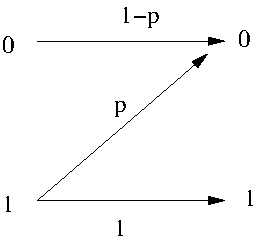
\includegraphics[scale=0.5]{capacidad/zchannel}
  \end{center}
  \caption{Diagrama: Z-channel}
  \label{fig:Gal}
\end{figure}

Para un Z-channel, la distribución de probabilidades de I(X;Y) es diferente \cite{Tallini:02}, por lo que obtenemos un máximo diferente:

\begin{equation}\label{CapA}
C_{Z} \approx 1 - \left(\frac{1}{2}*H(p)\right)
\end{equation}

Por lo tanto, expandiendo H(p) en \ref{CapA}:

$$ C_{Z} = \log_2\left(1+(1-p) p^{p/(1-p)}\right) $$

La diferencia entre las capacidades de ambos tipos de canal puede apreciarse fácilmente en la figura \ref{fig:CompBZ}, donde no tiene sentido hablar de una probabilidad de error mayor a 0.5 en un canal binario simétrico, es totalmente válido en un canal-Z y el mínimo de capacidad en este caso no es cuando $p=0.5$ sino cuando $p=1.0$.

\begin{figure}[th]
  \begin{center}
    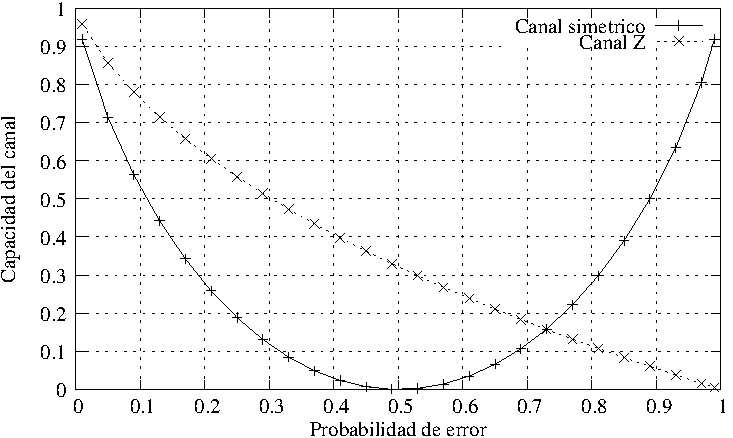
\includegraphics[scale=0.9]{graphs/grafico_comparacion_capacidad_binaria_z}
  \end{center}
  \label{fig:CompBZ}
\end{figure}


\section{Filtros de Bloom}
\label{bloomf}
Como se discutió en la sección \ref{Seguridad} , la colisiones de símbolos son inherentes a la modulación seleccionada.
En la modulación OOK utilizada en un medio óptico, solo los ‘1’s transmitidos pueden interferir con ‘0’s. Este comportamiento puede ser modelado como un canal-Z porque la superposición de pulsos de luz individuales representando ‘1’s puede solamente ser identificados como un ‘1’s, por que la interferencia solamente puede ser aditiva. De esto se desprende que un ‘0’ recibido es un signo inequívoco de la ausencia de pulsos en el slot de tiempo leído.
Una buena estructura para representar este tipo de datos es el filtro de Bloom \cite{Bloom70space/timetrade-offs}, que se utiliza generalmente en técnicas de hashing, utilizándolo para tests muy rápidos (O=1) de pertenencia de un miembro en un set.
La manera en que se implementó este algoritmo en el sistema propuesto se basa es copiar cada bit en K slots del frame transmitido, siendo el frame la representación física del filtro de Bloom.
En el extremo receptor es suficiente para recibir un solo ‘0’ entre las K copias del bit, para correctamente inferir que el bit original era originalmente un ‘0’, mientras que si el bit original era un ‘1’, las colisiones no tienen efecto debido a la naturaleza del canal-Z.

En la figura \ref{fig:bloomf} puede apreciarse gráficamente como se utiliza un filtro de Bloom para la transmisión de 12 clientes con una repetición $K=2$. Podría verse al algoritmo de filtro de Bloom como una técnica de CDMA, ya que también utiliza redundancia para lograr resistencia a interferencias.

\begin{figure}[th]
  \begin{center}
    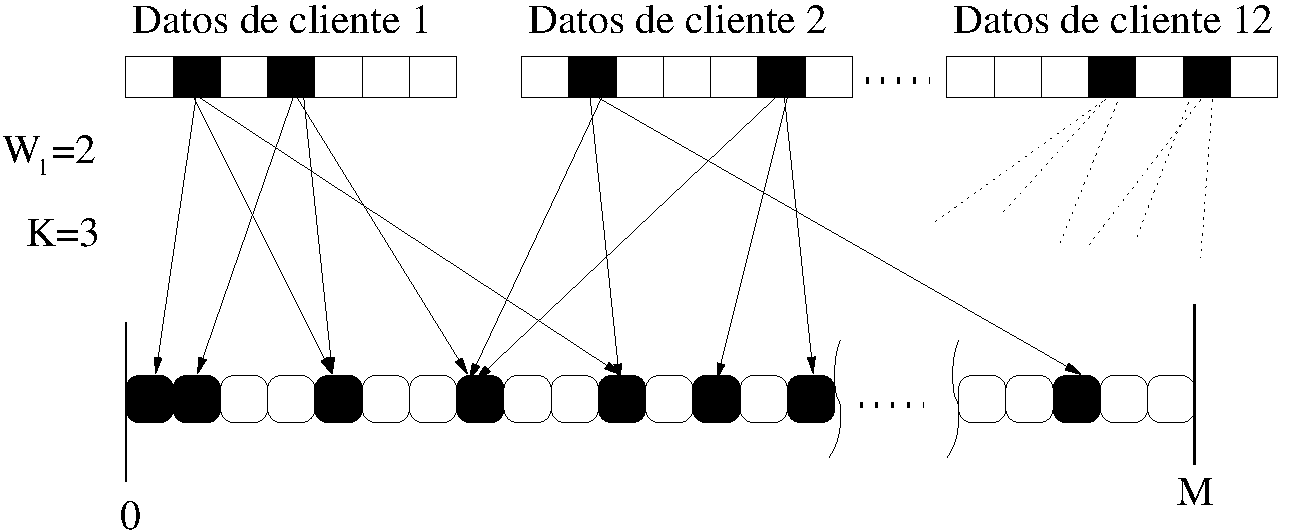
\includegraphics[scale=0.5]{frame-sp}
  \end{center}
  \caption{Filtro de Bloom}
  \label{fig:bloomf}
\end{figure}

%As discussed in section 2, this leads to collisions. Since the modulation format is OOK, only transmitted ‘1’s can interfere with ‘0’s.
%This behaviour can be modelled as a Z-channel because the superposition of individual light pulses representing ‘1’s
%can only be identified as a ‘1’, but a received ‘0’ is an unmistakable sign of the absence of pulses in a given time slot.
%We found that the Bloom filter [2] provides a convenient structure to correct for errors in this type of channel. This
%technique is borrowed from hashing algorithms and is used to test whether an element is member of a given set. The
%way that we implement this algorithm relies on copying every bit in K slots of the transmitted frame. On the receiving
%end it is sufficient to receive a single ‘0’ out of K copies in order to correctly retrieve the original transmitted ‘0’,
%whereas collisions have no effect on ‘1’s.

\subsection{Filtros de bloom encriptado: Time-hopping}

Es en esta etapa donde se logra la encriptación de los datos, reemplazando el algoritmo de hash que selecciona las posiciones de los datos dentro del filtro de Bloom por una función pseudo-aleatoria criptográficamente segura, de manera que los bits de datos de los diferentes clientes se ubican aleatoriamente en el frame y no es posible decodificarlos si no se posee la semilla del algoritmo PRNG, que equivale a la clave. Desde el punto de vista de modulación, como el algoritmo PRNG selecciona la posición dentro del frame, que es temporal, esto es equivalente a una transmisión Time-hopping, con la única salvedad que el algoritmo de filtro de Bloom requiere K repeticiones de los datos para poder recuperarse de colisiones en la recepción.

Para poder decodificar los datos en el filtro de Bloom receptor es necesario que todos los participantes posean la clave o semilla generadora del mismo PRNG utilizado para codificar los datos, y estar sincronizado a nivel de frame con el originante, para poder regenerar exactamente todas las posiciones en donde se transmitieron los datos. Los demás clientes solo causan interferencias que son corregidas primeramente por el filtro de bloom, y luego por el código de corrección de errores externo (Reed-Solomon por ejemplo), por lo tanto no es necesario que todos los clientes en la red estén sincronizados a nivel de frame, sino que solo es necesario para los clientes que deseen participar en el canal encriptado.

Es deseable pero no necesario que todos los clientes mantengan una sincronización a nivel de bit, de lo contrario un bit generalmente colisionará con dos bits en lugar de solo uno, y se necesitará aumentar la capacidad de corrección de errores del sistema.

\section{Minimización de peso de Hamming}
%% extraido de dline-pub.text

Repasando, el esquema propuesto basado en time-hopping CDMA se basa en la interferencia entre símbolos para obtener confidencialidad, ya que los datos de los otros usuarios actúan efectivamente como ruido.
La interferencia inter-símbolo, como fue discutida en la sección \ref{principle}, causa errores que debe ser corregidos. Como dichos errores reducen el ancho de banda utilizable del canal, es deseable reducir la interferencia hasta un punto donde se maximice, sin comprometer la seguridad del sistema. Para reducir la interferencia, no es aconsejable modificar o introducir patrones en el generador criptográficamente seguro de números aleatorios, ya que comprometería la seguridad de todo el sistema al introducir predictabilidad en las posiciones de los símbolos (Ej. usando códigos ortogonales como en Ref.~\cite{Nadarajah2006}.), efectivamente dejando de ser criptograficamente seguro.
En lugar de esto, se adopto una estrategia que aprovecha el echo que un sistema óptico puede ser modelado como un canal-Z.

%This channel presents a Shannon limit of $ C_{Z} = \log_2\left(1+(1-p) p^{p/(1-p)}\right),$ where $p$ is the probability of error~\cite{Tallini:02}.

Esta propuesta, el núcleo de la invención propuesta en esta tesis, es la de aprovechar la naturaleza asimétrica del este tipo de canal, en donde solamente el símbolo ``1'' causa interferencia, ya que los ``0'' no se interfieren. \footnote{Aunque en un sistema óptico real, existe efectivamente una pequeña diferencia ya que un ``0'' nunca es representado con una potencia de Laser de cero Watts.}
En otras palabras, la interferencia de un canal-Z es proporcional al peso de Hamming del símbolo transmitido.
El peso de Hamming de un símbolo es simplemente la cantidad de bits en ``1'' del mismo. El algoritmo de Minimización de peso de Hamming consiste en una codificación en donde cada símbolo binario es convertido en un equivalente de mayor longitud, teniendo solamente una mínima cantidad de dígitos en ``1''. Aplicando esta codificación que minimiza el peso de Hamming y transmitiendo el símbolo resultante, se obtiene una menor interferencia en un canal Z.
Intuitivamente, expandir el símbolo original a uno de mayor longitud decrementaría el ancho de banda del canal; pero como las simulaciones numéricas muestran (ver sección \ref{simulations}) a medida que la interferencia inter-símbolo se reduce, el ancho de banda adicional utilizado por los algoritmos de FEC también se reducen, compensando por el incremento del largo del símbolo y logrando un mayor ancho de banda neto del sistema.
Podemos decir que un número binario normal de largo L posee un peso variable de Hamming, con L/2 siendo el promedio, cero siendo el mínimo y L siendo el máximo peso de Hamming.
La técnica de reducción de peso de Hamming (HW) da buenos resultados reduciendo a HW=2, logrando un buen balance entre la reducción de interferencia y el largo de símbolo.
Adicionalmente, es deseable en un sistema de seguridad que no se revele ninguna información acerca de los símbolos transmitidos. Por ejemplo si transmitiéramos el número cero, representado por todos sus dígitos en cero, seria trivial identificarlo sin importar si se aplica cualquier tipo de time-hopping. Para evitar estos ataques que utilizan estadísticas acerca del peso de Hamming, la codificación exige que el peso de Hamming sea fijo en todos los símbolos. Esto causa una ligera perdida en el ancho de banda pero hace imposible inferir cualquier tipo de información acerca del símbolo transmitido analizando estadísticas de tráfico de los datos transmitidos.

\begin{table}[t]
\begin{center}
\begin{tabular}{c c c}
Datos & entrada HW= 0 to 3 & Expandida HW=2\\
\hline\hline
0 & 000 & 00011\\
1 & 001 & 00110\\
2 & 010 & 00101\\
3 & 011 & 01100\\
4 & 100 & 01010\\
5 & 101 & 01001\\
6 & 110 & 10001\\
7 & 111 & 10010\\
\end{tabular}
\caption{Tambla de minimización de Hamming para símbolos de 3-bits}
\label{hwtable}
\end{center}
 \end{table}
 
\section{Expansión de símbolo}
La minimización del peso de Hamming conlleva una necesaria conversión del símbolo original a otro que necesariamente tendrá mayor longitud, o sea, una expansión del símbolo.
Esta operación puede realizarse de muchas maneras, pero un algoritmo muy eficiente es utilizar una tabla de lookup (ver tabla~\ref{hwtable}), donde un símbolo de largo L es utilizado como el índice en la tabla, y el resultado es el símbolo expandido, que tiene un largo N\textgreater L.
Por motivos prácticos y de optimización, es deseable que L sea 8 u 16 bits, por lo que la tabla contendrá 256 o 65536 entradas respectivamente.
Al aplicar la minimización de peso de Hamming a símbolos de 8 o 16 bits de longitud, son necesarios 256 o 65536 símbolos de salida con un HW=2. En el caso de símbolos de entrada de 8 bits, la longitud del símbolo de salida sera de 363 bits, mientras que para 8 bits de entrada, el símbolo expandido con HW=2 tendrá 24 bits de longitud.
Puede observarse que el número de símbolos únicos con HW=2 y N=363 no es exactamente 65536 sino 65703, esto significa que la tabla de expansión no es única, sino que existen muchas tablas funcionalmente equivalentes que pueden seleccionarse para realizar la expansión.
La tabla seleccionada y el orden de la misma no son importantes para el resultado final, observando la condición que todos los nodos participantes de un canal deberán utilizar idénticas tablas.
%In general more bits transmitted per frame the more efficient the protocol will be. \textbf{PORQUE IN GENERAL? CUANDO FALLA?} 
\begin{figure}[!t]
  \centering
    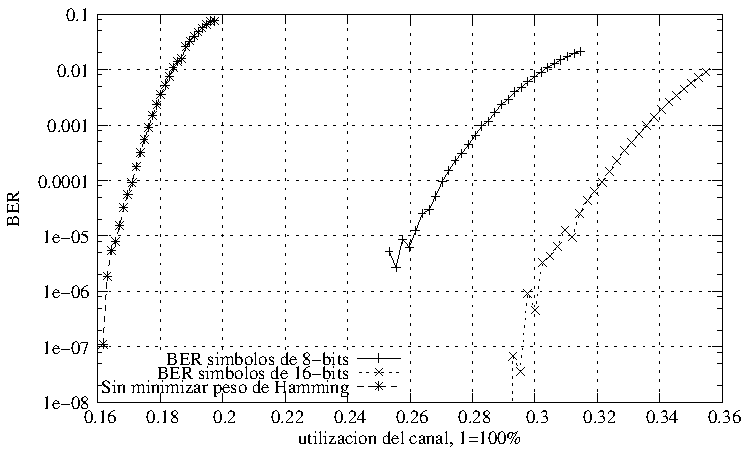
\includegraphics[width=6in]{graphs/BERvsChannelES2}
    \caption{Performance del sistema con respecto a la expansión de símbolo. Simulación numérica de un enlace de 10 Gbps con 128 clientes, M=4096 y K=9}
    \label{BERvsExpansion}
\end{figure}


\section{Probabilidad de colisión de filtro de bloom con expansión de símbolo}

%newJIS_140512
En esta sección, presentaremos una estimación analítica de la probabilidad de error de bit, tomando en cuento solo las interferencias de otros usuarios en la red.
Adicionalmente, no se considera ninguna corrección de etapas o algoritmos adicionales como Reed-Solomon, o interferencias producidas en el medio físico.
Como se explicó en \ref{bloomf}, asumiremos que cada usuario agrupa sus bits de información en paquetes o Frames, cada una de largo n. Cada paquete es codificado utilizando exactamente $m_{1}$ unos y $m_{0}$ ($m_{1}+m_{0}=m$. Cada uno de los $m$ dígitos binarios resultantes es repetido K veces en posiciones elegidas aleatoriamente en el frame de largo $M$. Repeticiones de un dígito binario puedes colisionar con otras repeticiones del mismo dígito, con repeticiones de otro dígito o bien con dígitos pertenecientes a otro cliente.
Llamaremos $N$ al número de usuarios activos. Para estimar la tasa de error o BER (Bit Error Rate) del sistema y simplificar los cálculos, haremos las siguientes asunciones:

\begin{enumerate}
 \item Asumiremos que los frames de diferentes usuarios están sincronizadas y cada frame contiene (incluyendo colisiones) $W_0 = N\cdot K\cdot m_0$ ceros y $W_1 = N\cdot K\cdot m_1$ unos.
 \item No incluiremos en el análisis la posibilidad de corrección de errores debido al echo que, en general, 
 \begin{equation}
\nchoosek{m}{m_1} > 2^n.
\end{equation}
Específicamente, cada vez que una secuencia errónea de $m$ dígitos binarios es recibida con mas de $m_1$ unos, se mapea a una cadena de bits aleatoria de largo $n$.
Por lo tanto, el número esperado de errores sera $n/2$.
\end{enumerate}

Bajo esas asunciones, el BER esta dado por
\begin{equation}
\text{BER} = \frac{n}{2}\prob{\text{sobre-escribir con unos las $K$ repeticiones de por lo menos uno de los $m_0$ ceros}}.
\label{eq:ber_01}
\end{equation}
Por la cota de la unión (union bound), 
\begin{multline}
\prob{\text{sobrescribir con unos las $K$ repeticiones de por lo menos uno de los $m_0$ ceros}}\leq \\
\leq m_0\prob{\text{sobrescribir con unos las $K$ repeticiones de uno de los $m_0$ ceros}}.
\label{eq:union_bound}
\end{multline}
Por lo tanto, prestemos atención a uno de los $m_0$ ceros. Si los $W_{1}$ transmitidos (por todos los usuarios) ocupan $s$ slots y las $K$ repeticiones del 0 dado usa $r ( \leq K)$ slots, entonces una condición necesaria para el error es que $s \geq r$. Por lo tanto asumamos que existen $s$ unos en un frame de $M$ bits. Dado $r$ lugares en el frame, la probabilidad de que los unos ocupen esas $r$ posiciones esta dada por 
\begin{equation}
z_{r,s} = \frac{\nchoosek{M-r}{s-r}}{\nchoosek{M}{s}}= \frac{\frac{(M-r)!}{(M-s)! (s-r)!}}{\frac{M!}{(M-s)!s!}} = \frac{(M-r)!}{M!}\frac{s!}{(s-r)!}\approx (\frac{s}{M})^r,
\end{equation}
Donde hemos asumido que $N,s\gg r$. Si $M \gg K$, no es difícil ver que las $K$ repeticiones de un cero dado ocupan $\mu_{R} \approx K$ slots en promedio. Tambien puede demostrarse que el número promedio de slots ocupados por los $W_{1}$ unos transmitidos por todos los usuarios es

\begin{equation}
\mu_{S} \approx M (1-e^{-W_1/M})
\end{equation}
 
Si $M$ y $W_{1}$ son grandes (ver apéndice TODO).
De esas ecuaciones, una estimación de la cota superior del BER para un determinado usuario es
\begin{equation}
\text{BER} \approx \frac{n}{2} m_0 z_{\bar{R},\bar{S}} \approx \frac{n}{2} m_0 \left(1-e^{-W_1/M}\right)^K.
\end{equation}

La figura \ref{BERvsK} muestra la estimación en función de $K$ para $M=2014$, $m_{0} = 22$, $m_{1} = 2$, $n = 8$ y $N=38$. Es interesante notar que existe un valor óptimo de la tasa de repetición $K$ que minimiza la tasa de error. Este resultado es relevante en el diseño de un sistema de comunicaciones. En particular, la última ecuación es muy simple y puede ayudar al diseño de red. Notar que los bajos valores de BER alcanzados permiten utilizar en la siguiente etapa algoritmos tales como Reed-Solomon, para reducir aun mas el BER total de sistema y asi llevarlo a tasas aceptables para las aplicaciones a las que este trabajo apunta.

\begin{figure}[!t]
  \centering
    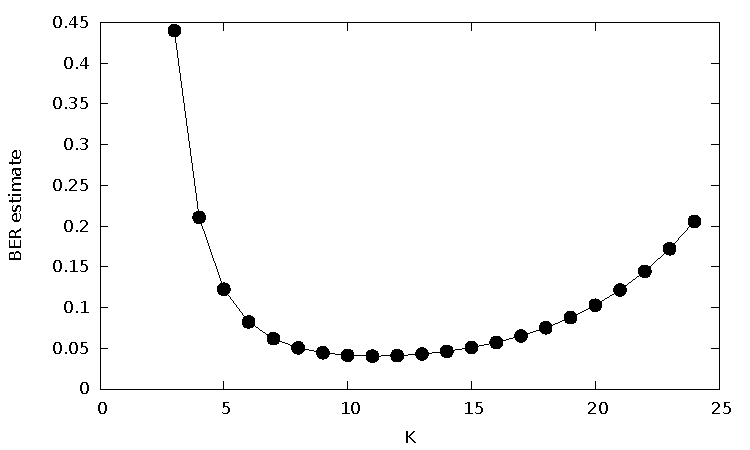
\includegraphics[width=5in]{Kcalc}
    \caption{Estimación de BER vs tasa de repetición de filtro de Bloom K.}
    \label{BERvsK}
\end{figure}

\section{Códigos de pseudo-ruido}
Como se explica en la sección \ref{PRNGs} la seguridad del sistema depende de la correcta selección e implementación de un algoritmo de PRNG criptográficamente seguro.
El sistema impone una restricción adicional a esta etapa, ya que además de cumplir con todas las propiedades de un CS-PRNG, se debe seleccionar un algoritmo eficiente ya que se necesitara generar una posición aleatoria por cada bit que se desea transmitir. Por lo tanto una característica que es deseable minimizar es la cantidad de bits por clock que el CS-PRNG es capaz de generar.
En el caso de la implementación para el transceptor óptico sobre una FPGA, el algoritmo seleccionado para el prototipo inicial fue el denominado ARC4, debido a la simplicidad, bajo consumo de recursos de hardware y alta velocidad del mismo. Si bien existen implementaciónes de alta performance \cite{10.1109/TC.2012.19}, estas no se encuentran disponibles al público general por lo que se implementó este algoritmo íntegramente en Verilog, utilizando optimizaciones para hacer llegar al algoritmo a la performance deseada de 1 byte de stream pseudoaleatorio por clock. Otro dato a tener en cuenta es que RC4 es un algoritmo relativamente anticuado, y recientemente varios ataques estadísticos han puesto en duda su utilización como generador criptográficamente seguro \cite{Sepehrdad:2011:SAR:2008684.2008712}, por lo que en implementaciones futuras es recomendable que sea reemplazado por un algoritmo mas adecuado.

En las implementaciones de software o acústicas los requerimientos para esta estapa se ven relajados desde el punto de vista de poder de procesamiento, ya que la velocidad de reloj de un CPU es tan elevada con respecto a la velocidad del medio que el PRNG seleccionado nunca se convierte en el cuello de botella en la pila de comunicaciones.

\section{Parámetro de seguridad}
(De Cryptograpy by V. V. IAshchenko)\cite{primes}

Para el análisis de complejidad de un sistema criptográfico se suele utilizar un parámetro variable que mide el tamaño del problema y representa a la vez los requerimientos del algoritmo criptográfico tanto como la probabilidad de un adversario de romper la seguridad en el sistema. Este es el llamado parámetro de seguridad, por ejemplo esto puede ser el largo de clave.
Este parámetro puede tomar valores arbitrariamente grandes.
Además, la definición de seguridad depende de la tarea que el adversario trata de realizar y de la información acerca del esquema criptográfico disponible.
Se suele especificar un valor en el cual la cantidad de cálculos necesarios por el atacante se presumen irrealizables, esto sera función del parámetro de seguridad seleccionado.
Según la tesis de Cobham\cite{citeulike:6647003}, el algoritmo del atacante se considera eficiente si esta limitado en tiempo polinomial sobra la longitud de la entrada (el parámetro de seguridad en este caso) de otra manera se considera inviable. Nótese que el algoritmo criptográfico en si mismo debe ser eficiente.

Finalmente se debe fijar un limite para la probabilidad despreciable. El contrato criptográfico estandard trata a la probabilidad como despreciable si no excede $\frac{1}{p(n)}$  para un polinomio $p$ y el parámetro de seguridad $n$.

Aceptadas esas cuatro definiciones, para probar que un algoritmo criptográfico es seguro basta con probar que la no-existencia de un algoritmo polinomial que realize la tarea del adversario.

De todas maneras, el estado actual de la teoría de complejidad no permite justificar un limite inferior de un problema como super-polinomial ($P=NP?$) por lo que la mayoría de las pruebas en el mundo de la seguridad están basadas en asunciones.
Por lo tanto, la investigación se concentra usualmente en buscar las condiciones suficientes mas débiles (o necesarios y suficientes) para la existencia de un esquema seguro.
Las asumciones son usualmente generales (Basadas en la teoría de complejidad) o basadas en intratabilidad de problemas en la teoría de números, etc.

\subsection{Aplicación al algoritmo de bloom-filter encriptado}

Este algoritmo puede verse como uno que a $r$ clientes le asigna $M$ posiciones de slot.
La cantidad posible de combinaciones de $M$ posiciones entre todos los clientes es de $ _{M}P_{r} = \frac{M!}{(n-r)!} $.
Definimos que el algoritmo se rompe cuando un atacante puede inferir la serie de posiciones $M$ para un cliente.

Existe un algoritmo de selección de $M$ que suponemos no posee ninguna debilidad, o sea, elije $r$ conjuntos de $M$ posiciones tal que teniendo una, no se pueda inferir otra.
El algoritmo seleccionado fue simplemente asignar a cada cliente su propio generador criptográficamente seguro, con claves diferentes para cada uno. Esto provocará colisiones pero para el cálculo del parámetro de seguridad se despreciará su efecto.

Suponemos:
\begin{itemize}
 \item El algoritmo de selección pseudoaleatorio no tiene debilidades.
 \item El atacante no posee control de los datos a transmitir, y estos son totalmente randomizados.
\end{itemize}

Dadas estas suposiciones (Equivalen a un ataque con plain-text desconocido en jerga criptográfica) para inferir el conjunto de posiciones $n$ de un cliente, el atacante deberá probar exhaustivamente todo el conjunto de $ _{M}P_{r}$ sobre una trama capturada, o bien probar todas las combinaciones posibles de la clave del generador pseudoaleatorio. De esto se desprende que con tener $clave>128\ bits$ y $M>128$ se puede asumir que el algoritmo cuenta con una seguridad denominada ``fuerte'', ya que una complejidad temporal de $2 ^{128}$ es considerada segura al momento de la escritura de esta tesis.

La segunda condición puede eliminarse con una cuidadosa selección de la tabla de expansión de Hamming, ya que al convertir los datos en símbolos uniformes con el mismo largo y el mismo peso de Hamming, no es necesario que los datos de entrada estén randomizados ya que aún si los datos de entrada son controlados por el atacante a la salida del Bloom-filter con expansión de símbolo siempre se observará también el mismo peso de Hamming\footnote{Mas correctamente, si el peso de Hamming es P, el atacante podrá observar un peso de Hamming de $1$ hasta $P$, debido a las colisiones de un cliente con sí mismo.} y el atacante no podrá inferir ninguna información de los datos de entrada.

\section{Resumen del sistema completo}
%% De orte.tex
El sistema propuesto, cuya estructura se aprecia en la figura \ref{fig_comstack}, esta compuesto primeramente de una capa de acceso, donde es implementada la codificación CDMA y corrección de errores, y una capa física basada o bien en una red óptica con similaridades a redes PON, o una red acústica de tipo broadcast.
La capa de acceso es implementada utilizando CDMA del tipo time-hopping, donde cada uno de los ONUs posibles codifica su información en bits y los envia en un slot seleccionado de manera aleatoria en un frame de $M$ slots\footnote{ Estos parámetros varían de acuerdo al nivel de error aceptable y cantidad de clientes máxima.}. De esta manera, ocurrirán múltiples colisiones entre diferentes ONUs pero serán subsanadas por la capa de corrección de errores que garantiza una transmisión de datos virtualmente\footnote{aunque es imposible eliminar totalmente los errores, un BER de 10E-12 se considera libre de errores} libre de errores.

Notar que la sincronización es realizada solo a nivel de bit-slot, en contraste con técnicas como TDMA que deben sincronizar a nivel de frame. También se elimina el requerimiento de una transmisión ordenada en el tiempo; en el esquema propuesto ambos clientes comunicantes pueden empezar su comunicación en cualquier momento, de manera similar al comportamiento del protocolo Ethernet.
Un cierto ONU $X$ puede recibir mensajes de otro ONU $Y$ si y solo si $X$ posee la {\em clave} de $Y$, y vice versa. De esta manera, si un cierto grupo de ONUs desean comunicarse sobre una VLAN encriptada, es requerido que cada uno en el grupo conozca la {\em clave}.

Los flujos de datos de las ONU's se codifican con las siguientes técnicas de corrección de errores:

Reed-Solomon ($223/255$) (ver \cite{Moon:05} y sus referencias), y un filtro de Bloom\cite{Bloom70space/timetrade-offs}. En principio un algoritmo LDPC ($1024\times512$ matrix) fue utilizado pero fue descartado en posteriores iteraciones del sistema, ya que al agregar la optimización de la expansión de símbolo al filtro de Bloom, se gano una capacidad de corrección adicional y pudo eliminarse el algoritmo LDPC de la pila de comunicaciones, con el consiguiente aumento de la capacidad total del sistema.

La selección de estos algoritmos de corrección de errores fue siempre considerando el canal de comunicaciones como el denominado canal Z. %que posee un limite de Shannon de $ C_{Z} = \log_2\left(1+(1-p) p^{p/(1-p)}\right),$ donde $p$ es la posibilidad de recibir un error al transmitir un bit. Este limite de capacidad es menor que el límite en una canal simétrico sin memoria \cite{Tallini:02}.

\section{Aplicación en distintos medios físicos}
La arquitectura del sistema lo hace muy confiable frente a interferencias de la capa física, al poseer una fuerte capacidad de recuperación de errores, por lo que modificando la etapa de modulación, pueden utilizarse diferentes medios físicos, siempre que tengan un modelo de ruido que se aproxime al canal Z.
\subsection{Redes ópticas}
% de orte.text


\begin{figure}[t]
  \centering
      \subfloat[Distribución via acoplador tipo estrella 1]{{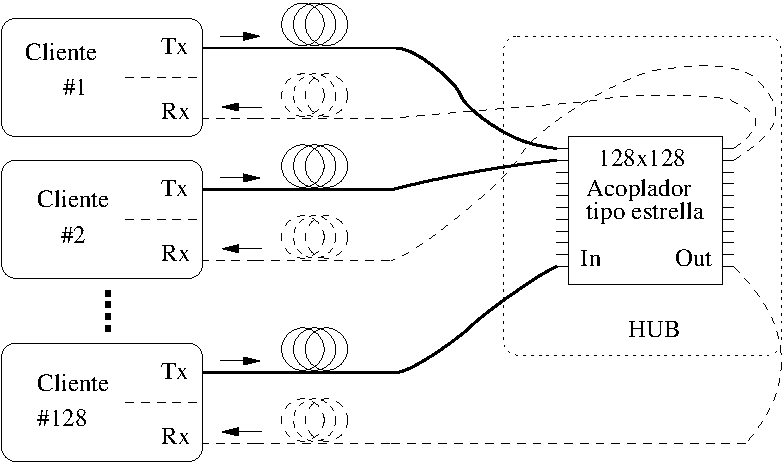
\includegraphics[width=0.45 \textwidth]{graphs/StarCoupler} }}%
    \qquad
    \subfloat[Distribución via EDFA]{{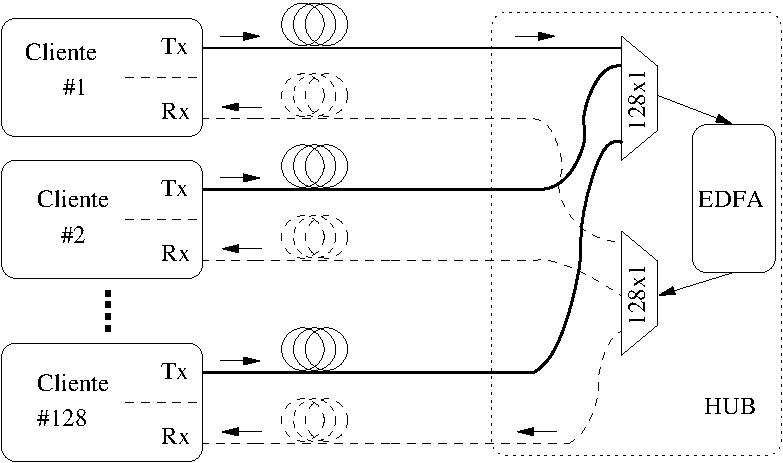
\includegraphics[width=0.45 \textwidth]{graphs/EDFA} }}%
    \caption{Diseño de red propuesto para la capa óptica: Un acoplador de tipo estrella es la base para la arquitectura de red en distancias inferiores a $10~\mathrm{km}$.}
    \label{arch:fig1}
\end{figure}

%\begin{figure}[t]
%  \centering
%  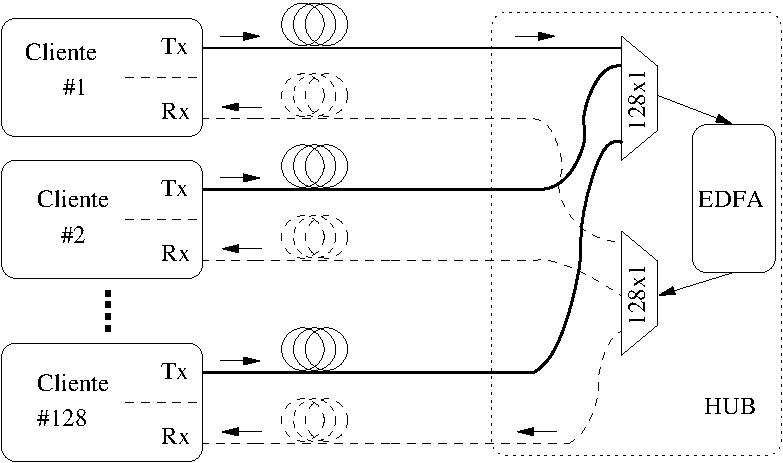
\includegraphics[width=0.48 \textwidth]{graphs/EDFA}
%  \caption{Para distancias superiores a $10~\mathrm{km}$ la red requiere amplificación provista por un EDFA.}
%  \label{arch:hub_edfa}
%\end{figure}


%\begin{figure}[!t]
%  \centering
%    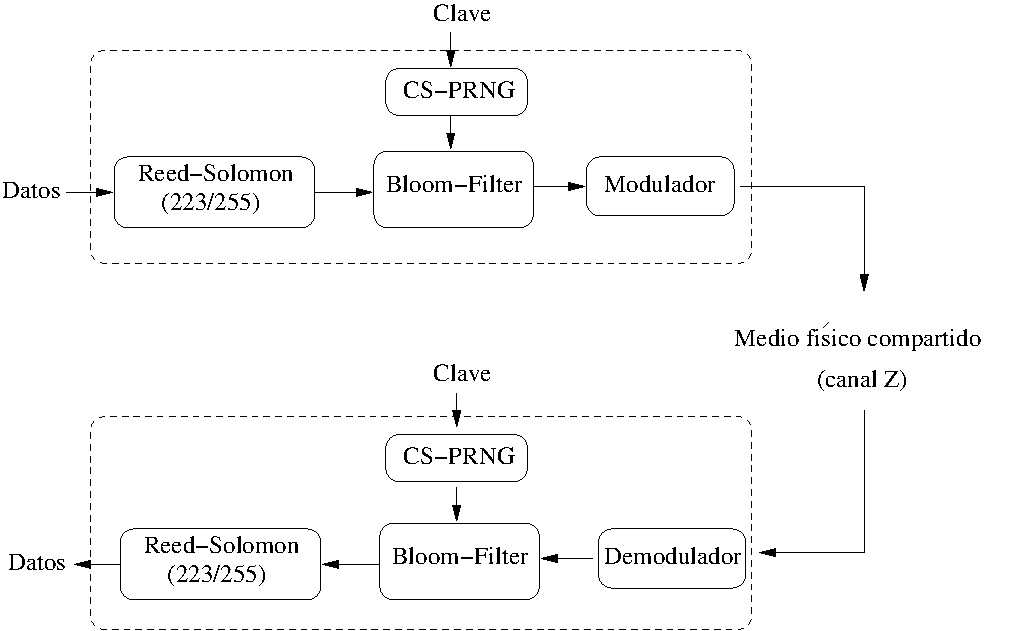
\includegraphics[width=5in]{graphs/Soft-stack3}
%    \caption{Diseño de red propuesto: Pila de comunicaciones}
%    \label{arch:chain}
%\end{figure}
% Fiber		Es grave el efecto de la dispersion?  Sugerimos dispersion shifted G.653? O son muy caras?
% splitter	No 1x128 commercially available (attenuation $\leq 27\,dB$)
% DFB		http://cess-dk.com/gfx/upload/PX2-1541SF.pdf ( min $\simeq-1\,dB$)
% APD		http://pdf.dzsc.net.cn/200810212/286762.pdf ( max $\simeq-27\,dB$)
% EDFA		http://www.lambdaphoto.co.uk/pdfs/EDFADatasheet.pdf

Al adaptar el sistema propuesto a una red óptica, la topología de misma debe ser de tipo estrella (ver Fig.\ref{arch:fig1}) donde splitters ópticos redistribuyen el tráfico proveniente de cada ONY a todo el resto permitiendo comunicaciones punto-a-punto asi como punto-a-multipunto entre hasta $128$ ONUs.
%Traffic redistribution is made by optical splitters at the redistribution hub that introduces high attenuation to optical streams.
Un amplificador óptico de fibra de Erbio (Erbium-Doped Fiber Amplifier, EDFA) localizado entre los splitters en el repetidor óptico incrementa la potencia óptica para contrarrestar las perdidas en la red, aunque esto es solamente necesario si el número de clientes es muy elevado o las pérdidas por dispersión son elevadas debido a las distancias entre ellos.

La modulación utilizada para las señales ópticas es RZ \footnote{La modulacíon RZ o ``Return to Zero'' es la mas común utilizada en fibras ópticas, aunque por razones técnicas en ralidad el laser nunca retorna a cero. Esto tiene consecuencias para el sistema propuesto como se vera mas adelante.} con velocidades previstas de hasta $10$~Gbps por un laser DBF de $2$~dBm de potencia y $1550$~nm de color/frecuencia. Estos parámetros permiten una transmisión de hasta $10$~km entre los nodos si se utiliza fibra óptica mono-modo estandard (ITU-T G.652) hacia el repetidor óptico.

En este hub, un spliter de $128\times 1$ maneja el tráfico de todos los ONUs y es luego redistribuido por el correspondiente splitter de $1\times 128$, canalizando el trafico mezclado de cada ONU a través de la fibra de bajada, paralela a la fibra de subida. Este splitter permite tener hasta 128 clientes o ONUs en el sistema. Si se requiere una menor cantidad, el splitter puede reducirse.
La atenuación de los splitters centrales ($\simeq25$~dB cada uno) sumado a la atenuación propia de la fibra óptica y perdidas por inserción ($\simeq2$~dB y $\simeq1$~dB por tramo) contribuyen a las altas pérdidas que este sistema debe compensar ($\simeq28$~dB en ambos canales de subida y bajada).

De utilizarse sin ningún tipo de amplificación, la atenuación que una señal sufriría entre dos ONUs es la suma de la atenuación de ambos tramos, o sea $\simeq56$~dB, que es un valor extremadamente alto fuera del alcance de la tecnología de detección disponible al momento de la escritura de esta tesis.

Sin embargo es posible pasar por etapas de amplificación intermedias para obtener niveles de señal adecuados. Para proveer la amplificación requerida, un EDFA con $\geq27$~dB de ganancia es colocado entre ambos splitters. Este EDFA incrementa la potencia del tráfico a la salida del primer splitter, elevando la potencia de cada '1' de $\simeq-26$~dBm a $1$~dBm a la entrada del segundo splitter, que sera reducida nuevamente por el mismo a un nivel de potencia de $-27$~dBm, que esta dentro de los parámetros aceptables de un foto-detector (PD) comercial de alta sensibilidad (Aprox. ($-28$~dBm)).

La potencia máxima de salida del PD no es un parámetro crítico ya que simulaciones [CUALES?] muestran que solamente se producirán colisiones de hasta diez `1' en un slot, y esto con una posibilidad extremadamente baja.

Aún considerando una ganancia de EDFA constante, la potencia de entrada óptica del PD seria menor ($-17$~dBm) que la que son capaces de soportar dispositivos comerciales ($\sim -5$~dBm).
El nivel de bit `0' es dado por la adición de todos los bits `0' transmitidos por todas las $128$~ONUs.
El nivel de decisión del receptor debería ser capaz de separar entre este estado y aquel de un simple ONU transmitiendo un solo bit en `1'.
De esto se desprende que la potencia de transmisión del bit `0' debe ser la menor posible, o lo que es lo mismo, el radio de extinción del Láser DBF debe ser alto.
El radio de extinción (`1'$/$`0' radio de potencia pico) mínimo requerido por el sistema se discute en las simulaciones numéricas a continuación:

% As collisions occur in this scheme minimal powers are such for the case of a single active Tx in a bit slot. In a bit slot with collisions (two or more `1' bits) power increase could be a concern to APD operation
% Optical transmission is performed by a $2$~dBm $1550$ nm DFB-laser generating a
% $10$ Gb/s RZ modulated optical signal, that is transported by up to $10$
% km upstream fiber (ITU-T G.652) to a redistribution hub (see
% Fig.~\ref{arch:fig1}).
% Upstream traffic from all ONUs are merged by a $128\times 1$ splitter and then again redistributed by another splitter $1\times 128$ that channels back merged traffic to each ONU through a downstream fiber identical and parallel to the upstream one.
% Splitters' attenuation ($\simeq25$~dB, estimated) contribute, as well as fiber attenuation and insertion losses ($\simeq2$~dB and $\simeq1$~dB per stretch), amount to high total attenuation ($\simeq28$~dB at each upstream and downstream paths).
% In order to make the system workable it is proposed to place a single EDFA optical amplifier ($\geq27$~dB gain) between both splitters.
% This EDFA rises merged traffic power at first splitter output ($\simeq-26$~dBm `1' active Tx) delivering enough power ($1$~dBm, `1' active Tx) at second splitter input to assure power reaching each ONU ($-27$~dBm, `1' active Tx) allows proper reception by a high sensitivity APD ($-28$~dBm).

\subsection{Redes acústicas}
% de newJIS_140512-1.pdf (paper JIS)
\begin{figure}[!t]
  \centering
    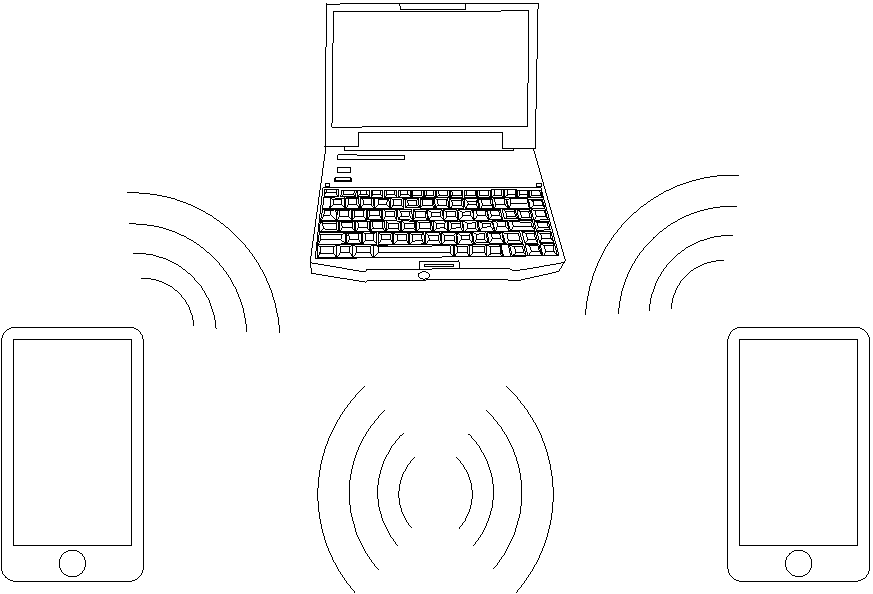
\includegraphics[width=3in]{compucelus.pdf}
    \caption{El diseño de red acústica propuesta puede contener nodos heterogéneos, tales como celulares móviles o computadoras personales.}
    \label{arch:chain}
\end{figure}

Un canal óptico es un claro ejemplo de canal Z, pero también es posible realizar un canal Z con redes acústicas si se utilizan ciertas modulaciones y parámetros.

Los enlaces ópticos presentan como mayor desventaja la necesidad de, o bien una fibra óptica entre los nodos comunicantes, o que exista visibilidad directa entre ambos nodos, una condición que no puede ser garantizada en muchos ambientes de trabajo. Además, los sensores ópticos requeridos generalmente no están presentes en los clientes y deben ser instalados separadamente.

Sin embargo utilizar un canal acústico tiene como ventaja poder utilizar hardware pre-existente en la mayoría de los potenciales clientes, como parlantes o micrófonos estandard, elementos muy comunes en dispositivos de información actuales \cite{citeulike:12800468}. Además, no es necesaria la visibilidad directa mientras ambos nodos estén localizados a pocos cm o metros de distancia, con bajo nivel de volumen.

Pero en contraste con otras tecnologías como RF o enlaces ópticos, la naturaleza del canal de sonido y la facilidad para interceptar o registrar comunicaciones utilizando este medio hace necesaria que la privacidad sea un requerimiento esencial. Muchos sistemas de comunicación de audio han sido propuestos \cite{august2002apparatus}, pero hasta donde fue posible investigar, el problema de la privacidad en este tipo de comunicaciones ha sido solucionada solamente en la capa de aplicación, o sea en alto nivel. Este trabajo presenta una aproximación a la seguridad y privacidad desde la capa física, basada también en time-hopping CDMA, similar a aquella presentada en \cite{6476559}. En este trabajo se presenta una red segura acústica punto-a-punto y punto-a-multipunto de corto rango y bajo consumo, que no requiere de ningún hardware adicional en clientes móviles.
Establecer un enlace privado entre dispositivos móviles previamente desconectados requiere cierto nivel de interacción por parte del usuario que es usualmente ignorado \cite{4912753}. Sin embargo, cuando la privacidad se brinda desde la capa física, la intervención del usuario es minimizada. Este es el caso de esta propuesta.

Un escenario válido para la aplicación de esta tecnología podría ser la validación de transacciones financieras pequeñas tales como terminales PoS (Point of Sale) o cajeros automáticos (ATM) utilizando un dispositivo móvil (Ej. un smartphone) sin modificaciones de hardware. Una tecnología similar que se utiliza en estos casos es la denominada Near Field Communications (NFC) [10], un protocolo inalámbrico que requiere hardware especializado que al momento de escritura de esta tesis no se encuentra disponible en la mayoría de los dispositivos móviles.
Es necesario ajustar algunos parámetros con respecto a la implementación óptica. Especialmente el tamaño de frame que se reduce de $M=4096$ a $M=256$ para la implementación óptica y un $K=9$ que es el óptimo para el $M$ seleccionado. El número de clientes también se ve reducido de $N=128$ a $N=12$ ya que al ser la red acústica de relativo corto alcance, no se prevé una elevada cantidad de clientes simultáneos. En la figura \ref{arch:AudioSimul} puede verse una simulación del sistema con estos parámetros contrastada con una medición realizada entre una Notebook (T420) y un celular (Lenovo A789).

\begin{figure}[t]
  \centering
    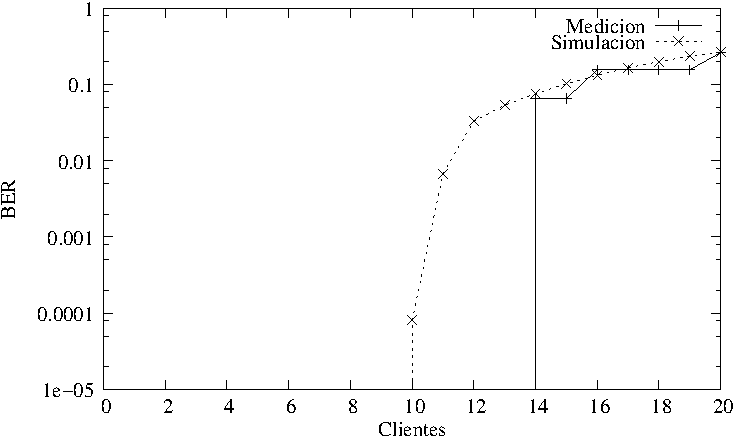
\includegraphics[width=4in]{graphs/audio-fig6}
    \caption{Sn M=256 y K=9}
    \label{arch:AudioSimul}
\end{figure}



\subsection{Redes acústicas: Arquitectura}

Una ventaja muy importante del sistema acústico propuesto es su simplicidad, requiriendo solamente un emisor de sonido (parlante), un receptor (micrófono) y un canal de transmisión de sonido que puede ser aire (y en casos mas especializados, agua). Ambos requerimientos están generalmente disponibles en computadoras, notebooks, tablets y teléfonos celulares modernos. 
El esquema lógico es el mismo que el descrito anteriormente: Time-hopping CDMA seguro, códigos correctores de errores y un método de sincronización a nivel de bit.
Como resultado, el sistema provee canales unidireccionales a los usuarios que sirven tanto para comunicaciones punto-a-punto como punto-a-multipunto. Comunicaciones bi-direccionales pueden establecerse utilizando dos canales separados (Ej. utilizando dos códigos CDMA diferentes), o empleando el mismo canal de manera half-duplex, aunque este último modo de funcionamiento necesita de desarrollo adicional y no es el objetivo de esta tesis.
En las próximas secciones se describe el sistema en mayor detalle.

\subsection{Redes acústicas: Modulación y sincronización}
\begin{figure}[t]
  \centering
    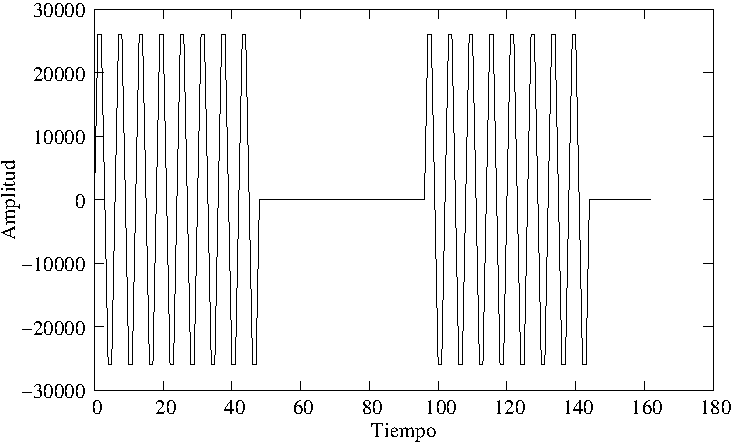
\includegraphics[width=4.5in]{graphs/modulated.pdf}
    \caption{Modulación OOK}
    \label{arch:sync}
\end{figure}


A diferencia de la implementación óptica, fue necesario implementar tanto el algoritmo de modulación acústica como el de sincronización.
Para la modulación, fue utilizado el algoritmo de On-Off Keying, que codifica los bits a transmitir como pulsos. La frecuencia de portadora puede variar de 10 kHz a 16 kHz, y buenos resultados se obtienen con una tasa de transferencia de 1000 bps. Nótese la baja velocidad de este canal, que introduce un problema inexistente en la implementación óptica: el retraso de la red (El tiempo que tarda un bit en atravesar toda la red) es alto, debido principalmente a la etapa de Reed-Solomon que necesita recibir 256 bits para poder empezar a decodificar, esto sumado a que el canal solo puede soportar 1000 bps, la baja velocidad del mismo y que es un medio compartido, eleva el retraso a niveles inaceptables, del orden de los 30 segundos.
Una selección mas apropiada del algoritmo de FEC (tal como BCH \cite{Moon:05}) podría drásticamente reducir el retraso total del sistema.
Adicionalmente, una etapa de pulse-shaping se agrega utilizando un filtro pasa-banda a la salida de la modulación y también en la entrada del demodulador. Este filtro adicionalmente ayuda a rechazar interferencia acústica o ruido ambiente.

\begin{figure}[t]
  \centering
    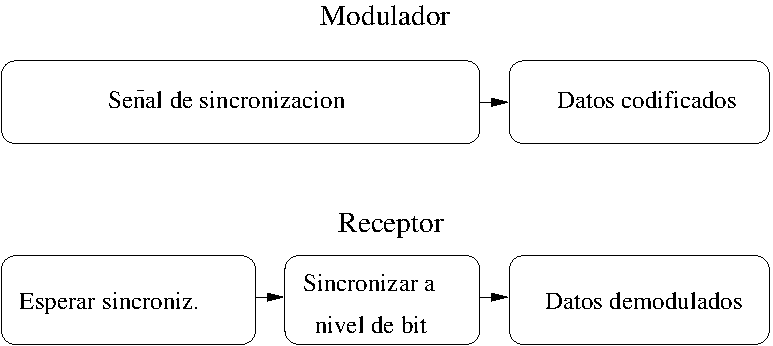
\includegraphics[width=4in]{graphs/Audio-Sync2.pdf}
    \caption{Sincronización}
    \label{arch:sync}
\end{figure}



La sincronización entre un transmisor y un receptor es esencial para la decodificación correcta de la información. Por esta razón, un patrón de sincronización inicial es enviado, para que el receptor pueda ajustar parámetros tales como la fase y nivel de decisión del la señal (ver Fig. \ref{arch:sync}). La deriva (Drift) del reloj y variabilidad (Jitter) no son significativas a esta velocidad de transmisión tan lenta y ninguna corrección en tiempo real es requerida, por lo que la implementación del módem por software es simple.
El nivel de decisión del demodulador es dinámico, o sea que es constantemente recalculado utilizando los niveles de entrada promediados.
La fase del símbolo recibido también es corregida utilizando los mismos datos de entrada como referencia.

